\providecommand{\rvCorner}[1]{\ulcorner #1\urcorner} %

\section{宇宙论函子再访}\label{sec:cosmological-functors-revisited}

请回忆\cref{def:cosmological-functor}：\textbf{\trCosmologicalFunctor}是诸%
\trInfinityCosmos{}之间的一个\trSimplicialFunctor{} $F\colon\mathcal{K}\to\mathcal{L}$，
它保持
\begin{itemize}
\item 指定的诸\trIsofibration{}类，以及
\item 全部宇宙论\trLimit。
\end{itemize}
\cref{lem:cosmological-preserves-equivalences}表明，\trCosmologicalFunctor{}还%
保持诸\trEquivalence{}与诸\trTrivialFibration{}。由\cref{prop:flexible-weights-homotopical}(i)，
\trCosmologicalFunctor{}还保持全部\trFlexibleWeightedLimit。

\trCosmologicalFunctor{}的例子比比皆是——例如见\cref{prop:cosmological-functor-constructions}，
以及 6.3 节中构造的诸充盈子\trInfinityCosmos{}之\trCosmologicalEmbedding。
还有一些\trCosmologicalFunctor{}，连接着以\trInverseCategory{}为指标的\trFibrant\trDiagram{}之%
诸\trInfinityCosmos{}（见练习 6.1.iii），例如

定义域\trFunctor、余定义域\trFunctor{}与恒同\trFunctor
\begin{center}
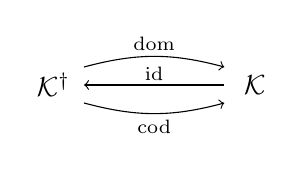
\begin{tikzpicture}[x=1.3em,y=1.3em]
  \node (Kd) at (0,0) {$\mathcal{K}^{\dagger}$};
  \node (K) at (5.6,0) {$\mathcal{K}$};
  \draw[->] (0.85,0.5) to[bend left=15] (4.75,0.5);
  \node at (2.8,1.15) {$\scriptstyle\mathrm{dom}$};
  \draw[->] (4.75,0) -- (0.85,0);
  \node at (2.8,0.32) {$\scriptstyle\mathrm{id}$};
  \draw[->] (0.85,-0.5) to[bend right=15] (4.75,-0.5);
  \node at (2.8,-1.15) {$\scriptstyle\mathrm{cod}$};
\end{tikzpicture}
\end{center}
而\cref{prop:isofibration-cosmos}证明了这些\trFunctor{}是宇宙论的。

\trCosmologicalFunctor{}常常可以限制，从而在平行的充盈子\trInfinityCosmos{}之间%
定义出进一步的\trCosmologicalFunctor：

\begin{lemma}\label{lem:restrict-replete-cosmological}
设 $\mathcal{K}'\hookrightarrow\mathcal{K}$ 与 $\mathcal{L}'\hookrightarrow\mathcal{L}$
是诸充盈子\trInfinityCosmos{}的\trCosmologicalEmbedding。若 $F\colon\mathcal{K}\to\mathcal{L}$
是一个\trCosmologicalFunctor，它把 $\mathcal{K}'$ 的对象与 0-箭头送到
$\mathcal{L}'$ 的对象与 0-箭头，则限制所得的\trFunctor{}是\trCosmological：
\begin{center}
\begin{tikzpicture}[x=1.3em,y=1.3em]
  \node (Kp) at (0,1.2) {$\mathcal{K}'$};
  \node (Lp) at (5.2,1.2) {$\mathcal{L}'$};
  \node (K)  at (0,-1.2) {$\mathcal{K}$};
  \node (L)  at (5.2,-1.2) {$\mathcal{L}$};
  \draw[->,dashed] (0.75,1.2) -- node[above]{$\scriptstyle F$} (4.45,1.2);
  \draw[right hook->] (0,0.7) -- (0,-0.7);
  \draw[right hook->] (5.2,0.7) -- (5.2,-0.7);
  \draw[->] (0.75,-1.2) -- node[below]{$\scriptstyle F$} (4.45,-1.2);
\end{tikzpicture}
\end{center}
\end{lemma}

\begin{proof}
请回忆，\cref{def:replete-subcategory}的充盈性包含如下要求：包含
$\mathcal{K}'\hookrightarrow\mathcal{K}$ 与 $\mathcal{L}'\hookrightarrow\mathcal{L}$
在正维箭头上为满。于是，若\trSimplicialFunctor{} $F$ 把 $\mathcal{K}'$ 的对象与
0-箭头送到 $\mathcal{L}'$ 的对象与 0-箭头，则它限制而定义一个%
\trSimplicialFunctor{} $F'\colon\mathcal{K}'\to\mathcal{L}'$。由于诸%
\trCosmologicalEmbedding{}创造\trIsofibration{}与诸\trCosmologicalLimitNotions，
限制所得的\trFunctor{}是\trCosmological。
\end{proof}

例如，由命题 5.2.4 与练习 5.3.i，\trPullback{}
$f^{*}\colon\mathcal{K}_{/B}\to\mathcal{K}_{/A}$ 保持\trCartesianFibration{}与%
\trCartesianFunctor。于是，沿 $\mathcal{K}$ 中任何\trFunctor{}
$f\colon A\to B$ 的\trPullback{}都限制而定义一个\trCosmologicalFunctor{}（见
命题 7.2.4）：
\begin{center}
\begin{tikzpicture}[x=1.3em,y=1.3em]
  \node (Cl) at (0,1.2) {$\mathcal{C}\mathit{art}(\mathcal{K})_{/B}$};
  \node (Cr) at (7.8,1.2) {$\mathcal{C}\mathit{art}(\mathcal{K})_{/A}$};
  \node (Kl) at (0,-1.2) {$\mathcal{K}_{/B}$};
  \node (Kr) at (7.8,-1.2) {$\mathcal{K}_{/A}$};
  \draw[->,dashed] (Cl) -- node[above]{$\scriptstyle f^{*}$} (Cr);
  \draw[right hook->] (0,0.55) -- (0,-0.55);
  \draw[right hook->] (7.8,0.55) -- (7.8,-0.55);
  \draw[->] (Kl) -- node[below]{$\scriptstyle f^{*}$} (Kr);
\end{tikzpicture}
\end{center}

本节的目标是表明：\trCosmologicalFunctor{}保持我们已引入的全部∞-范畴论结构
——仅有一个值得注意的例外，将在\cref{war:composites-not-preserved}中讨论。
在许多情形下，这一点从原本的 2-范畴式定义（例如定义 5.2.1 中%
\trCartesianFibration{}的定义）来看并不显然，但却可以相当容易地从每个范畴论
概念相配套的「内部刻画」（如定理 5.2.8(ii) 所给者）推出。

重要的是：

\begin{proposition}\label{prop:comma-infinity-categories-preserved}
\trCosmologicalFunctor{}保持\trCommaInfinityCategory：若
$F\colon\mathcal{K}\to\mathcal{L}$ 是一个\trCosmologicalFunctor，且左下图是
$\mathcal{K}$ 中的一个\trCommaCone，则右下图是 $\mathcal{L}$ 中的一个%
\trCommaCone。
\begin{rveq}\label{eq:comma-cone-under-F}
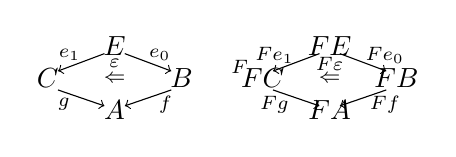
\begin{tikzpicture}[x=1.05em,y=1.05em]
  \begin{scope}
    \node at (0,2.2)    {$E$};
    \node at (-2.3,1.1) {$C$};
    \node at (2.3,1.1)  {$B$};
    \node at (0,0)      {$A$};
    \draw[->] (-0.35,1.95) -- (-1.95,1.35);
    \node at (-1.55,1.9)  {$\scriptstyle e_{1}$};
    \draw[->] (0.35,1.95) -- (1.95,1.35);
    \node at (1.55,1.9)   {$\scriptstyle e_{0}$};
    \node at (0,1.6)      {$\scriptstyle\varepsilon$};
    \node at (0,1.1)      {$\scriptstyle\Leftarrow$};
    \draw[->] (-1.95,0.7) -- (-0.35,0.15);
    \node at (-1.75,0.2)  {$\scriptstyle g$};
    \draw[->] (1.95,0.7) -- (0.35,0.15);
    \node at (1.75,0.2)   {$\scriptstyle f$};
  \end{scope}
  \node at (4.3,1.5)  {$\scriptstyle F$};
  \node at (4.3,0.85) {$\scriptstyle\rightsquigarrow$};
  \begin{scope}[shift={(7.4,0)}]
    \node at (0,2.2)    {$FE$};
    \node at (-2.3,1.1) {$FC$};
    \node at (2.3,1.1)  {$FB$};
    \node at (0,0)      {$FA$};
    \draw[->] (-0.35,1.95) -- (-1.95,1.35);
    \node at (-1.9,1.9)   {$\scriptstyle Fe_{1}$};
    \draw[->] (0.35,1.95) -- (1.95,1.35);
    \node at (1.9,1.9)    {$\scriptstyle Fe_{0}$};
    \node at (0,1.6)      {$\scriptstyle F\varepsilon$};
    \node at (0,1.1)      {$\scriptstyle\Leftarrow$};
    \draw[->] (-1.95,0.7) -- (-0.35,0.15);
    \node at (-1.9,0.2)   {$\scriptstyle Fg$};
    \draw[->] (1.95,0.7) -- (0.35,0.15);
    \node at (1.9,0.2)    {$\scriptstyle Ff$};
  \end{scope}
\end{tikzpicture}
\end{rveq}
\end{proposition}

\begin{proof}
构造\trCommaCone{}的那个单纯\trPullback{} (3.4.2) 为任何\trCosmologicalFunctor{}所保持。
由命题 3.4.11，任何如上方左图所示的\trCommaCone{}都从一支\trFiberedEquivalence
$\rvCorner{\epsilon}\colon E\simeq_{C\times B}\mathrm{Hom}_{A}(f,g)$ 产生，其中
$\epsilon=\phi\rvCorner{\epsilon}$，而任何这种形式的\trFiberedEquivalence{}都%
定义一个\trCommaCone。由于 $F$ 定义一个\trCosmologicalFunctor{}
$F\colon\mathcal{K}_{/C\times B}\to\mathcal{L}_{/FC\times FB}$，故有
$F\rvCorner{\epsilon}\colon FE\simeq_{FC\times FB}F(\mathrm{Hom}_{A}(f,g))\cong\mathrm{Hom}_{FA}(Ff,Fg)$，
于是我们得出结论：右图的数据同样定义一个\trCommaCone。
\end{proof}

利用\cref{prop:comma-infinity-categories-preserved}，我们可以迅速确立%
\trCosmologicalFunctor{}的下列保持性质。为便于查检，这张清单也把在别处确立的
保持性质一并收入。

\begin{proposition}\label{prop:cosmological-preservation-properties}
\trCosmologicalFunctor{}保持：
\begin{enumerate}[label=(\roman*)]
\item \trInfinityCategory{}之间的\trEquivalence。
\item 可逆\trNaturalTransformation{}与对应。
\item \trInfinityCategory{}之间的\trAdjunction，包括右伴随右逆伴随与左伴随
  右逆伴随。
\item \trFiberedAdjunction{}与\trFiberedEquivalence。
\item \trIsofibration、\trTrivialFibration{}与\trDiscrete{}\trInfinityCategory。
\item \trFlexibleWeightedLimit。
\item \trCommaSpan{}与\trCommaCone。
\item \trAbsoluteRightLifting{}图表与\trAbsoluteLeftLifting{}图表。
\item 以\trSimplicialSet{}为指标的\trDiagram{}之\trLimit{}或\trColimit，
  以及保余极限/保极限的\trFunctor。
\item \trStable{}\trInfinityCategory{}与\trExactFunctor。
\item \trCartesianFibration{}与\trCocartesianFibration，以及其间的%
  \trCartesianFunctor。
\item \trDiscreteCartesianFibration{}与\trDiscreteCocartesianFibration。
\item \trTwoSidedFibration，以及其间的\trCartesianFunctor。
\item \trModule{}与可表示模。
\end{enumerate}
\end{proposition}

\begin{proof}
由\cref{lem:simplicial-functor-2-functor}，一个\trCosmologicalFunctor{}诱导诸%
\trHomotopyTwoCategory{}之间的一个 2-\trFunctor，而任意的 2-\trFunctor{}都保持
(i)、(ii) 与 (iii) 的诸结构（例如见引理 2.1.3）。由于\trCosmologicalFunctor{}在
诸\trSliceInfinityCosmos{}之间诱导\trCosmologicalFunctor，(iv) 可以理解为
(i) 与 (iii) 的特例。

\trTrivialFibration{}的保持已由\cref{lem:cosmological-preserves-equivalences}
确立，而\trDiscrete{}\trInfinityCategory{}的保持随之得出（见%
\cref{rem:cosmological-discrete-categories}）。\cref{prop:flexible-weights-homotopical}(i)
证明\trCosmologicalFunctor{}保持全部\trFlexibleWeightedLimit，即 (vi) 所述。
\cref{prop:comma-infinity-categories-preserved}证明\trCosmologicalFunctor{}保持%
\trInfinityCosmos{}中的\trCommaSpan{}与\trHomotopyTwoCategory{}中的\trCommaCone，
即 (vii) 所述。

保持性质 (viii) 最先见于推论 3.5.7，它由定理 3.5.3（该定理把绝对提升图表刻画
为逗号∞-范畴之间的\trFiberedEquivalence）、\cref{prop:comma-infinity-categories-preserved}
（它说\trCosmologicalFunctor{}保持诸逗号）以及「\trCosmologicalFunctor{}保持诸%
\trEquivalence」这一事实得出。(ix) 则由这一点、定义 2.3.8 以及「%
\trCosmologicalFunctor{}保持单纯\trTensor」这一事实得出，其中关于保余极限/
保极限\trFunctor{}的陈述由 (ii) 得出。由定理 4.4.12(iii)，(x) 可以理解为
(ix) 的特例。

保持性质 (xi) 与 (xii) 也由\cref{prop:comma-infinity-categories-preserved}得出
——经由定理 5.2.8(ii)、定理 5.3.4(ii) 与命题 5.5.8 的诸刻画，加上「%
\trCosmologicalFunctor{}保持右或左伴随右逆伴随、对应与\trTrivialFibration」
这一事实。更多细节见推论 5.3.5 的证明；该证明还观察到，笛卡尔自然变换亦为%
\trCosmologicalFunctor{}所保持。

直接从定理 7.1.4 的内部刻画以及伴随与可逆\trNaturalTransformation{}的保持出发，
可得：\trCartesianFunctor{}保持\trTwoSidedFibration{}与其间的\trCartesianFunctor，
如推论 7.1.8 所观察。这就确立了 (xiii)。由\cref{prop:cosmological-functor-constructions}(vi)，
一个\trCosmologicalFunctor{}在诸\trSliceInfinityCosmos{}之间诱导一个直像%
\trCosmologicalFunctor，后者再由 (v) 保持离散对象。于是，\trModule{}也被保持。
把\cref{prop:comma-infinity-categories-preserved}特化到含恒同的\trCospan，
立见左可表示逗号与右可表示逗号被保持。由于一支\trModule{}是可表示的，当且仅当
它与其中之一纤维化等价，可表示\trModule{}也随之被保持——这就完成了 (xiv) 的
证明。
\end{proof}

\begin{warning}\label{war:composites-not-preserved}
在\trCosmologicalFunctor{}所保持的∞-范畴论结构清单中，显著缺席者是模的%
\trVirtualEquipment{}中的诸复合，以及参照这一概念而定义的种种进一步结构：
\trExactSquare、逐点右\trExtension{}与左\trExtension，以及以∞-范畴为指标的%
\trDiagram{}之（加权）\trLimit{}与\trColimit。

复合与强复合一般不为\trCosmologicalFunctor{}所保持，这背后有多种因素。一个
立即可见的问题出自定义 8.3.1 与定义 8.3.5 所给的诸\trUniversalProperty：
其中每一条都涉及全称量词。由于\trCosmologicalFunctor{}未必\trEssentiallySurjective，
定义域中的全称量词未必辖及余定义域。

在另一些语境中，全称量词可以借诸∞-范畴论概念的「内部刻画」而免除，但本情形
没有给出这样的刻画。症结在于这样一个事实：复合的\trModule{}应当理解为借一个
「拉回稳定的逐纤维余反转器」而定义，这一构造把由诸\trSpan{}之复合构成的%
\trTwoSidedFibration{}反射为\trDiscrete{}双侧纤维化。我们未曾给出这样的构造，
因为我们关于\trInfinityCosmos{}的公理化概念不包含余极限；但即便包含——而且
题外话 E.1.8 表明，∞-范畴的\trHomotopyColimit{}在诸例子中常常存在——%
\trCosmologicalFunctor{}由于其「类右伴随」的品性，也不会保持它们。

话虽如此，凡由应用引理 8.3.7 而得的强复合都为\trCosmologicalFunctor{}所保持，
因为\trFiberedAdjunction{}被保持。这包括 8.3 节与 8.4 节所确立的全部形式地定义的复合。
类似的评论也适用于\trExactSquare。由于一般的复合不为\trCosmologicalFunctor{}所
保持，一般的\trExactSquare{}也未必被保持。但 9.2 节所确立的形式地定义的诸%
\trExactSquare{}为\trCosmologicalFunctor{}所保持。例如，\cref{lem:comma-squares-exact}
证明：\trCommaSquare{}在任何\trInfinityCosmos{}中都是\trExactSquare。由于%
\trCosmologicalFunctor{}保持\trCommaSquare，这一类\trExactSquare{}便随之被保持。

正如我们将发现的，\trCosmologicalBiequivalence{}\emph{确实}保持全部这些
∞-范畴论概念，而且还反射并创造它们。我们现在就转向这一主题。
\end{warning}

\subsection*{练习}

\begin{exercise}\label{ex:sliced-fib-cosmos-functor}
请论证：任何\trCosmologicalFunctor{} $F\colon\mathcal{K}\to\mathcal{L}$ 都对
$\mathcal{K}$ 中的每一对\trInfinityCategory{} $A$ 与 $B$ 诱导一个%
\trCosmologicalFunctor{}
$F\colon{}_{A}\mathcal{F}\mathit{ib}(\mathcal{K})_{/B}\to{}_{FA}\mathcal{F}\mathit{ib}(\mathcal{L})_{/FB}$。
\end{exercise}

\begin{exercise}\label{ex:reflected-created-properties}
练习 6.3.iv 表明，\trCosmologicalEmbedding{}在保持\trDiscrete{}\trInfinityCategory{}%
之外还反射它们。\trCosmologicalEmbedding{}还反射或创造哪些其他的∞-范畴论性质？
\end{exercise}

